%%%%%%%%%%%%%%%%%%%%%%% file template.tex %%%%%%%%%%%%%%%%%%%%%%%%%
%
% This is a general template file for the LaTeX package SVJour3
% for Springer journals.          Springer Heidelberg 2010/09/16
%
% Copy it to a new file with a new name and use it as the basis
% for your article. Delete % signs as needed.
%
% This template includes a few options for different layouts and
% content for various journals. Please consult a previous issue of
% your journal as needed.
%
%%%%%%%%%%%%%%%%%%%%%%%%%%%%%%%%%%%%%%%%%%%%%%%%%%%%%%%%%%%%%%%%%%%
%
% First comes an example EPS file -- just ignore it and
% proceed on the \documentclass line
% your LaTeX will extract the file if required
\begin{filecontents*}{example.eps}
%!PS-Adobe-3.0 EPSF-3.0
%%BoundingBox: 19 19 221 221
%%CreationDate: Mon Sep 29 1997
%%Creator: programmed by hand (JK)
%%EndComments
gsave
newpath
  20 20 moveto
  20 220 lineto
  220 220 lineto
  220 20 lineto
closepath
2 setlinewidth
gsave
  .4 setgray fill
grestore
stroke
grestore
\end{filecontents*}
%
\RequirePackage{fix-cm}
%
%\documentclass{svjour3}                     % onecolumn (standard format)
%\documentclass[smallcondensed]{svjour3}     % onecolumn (ditto)
\documentclass[smallextended]{svjour3}       % onecolumn (second format)
%\documentclass[twocolumn]{svjour3}          % twocolumn
%
\smartqed  % flush right qed marks, e.g. at end of proof
%
\usepackage{graphicx}

%
% \usepackage{mathptmx}      % use Times fonts if available on your TeX system
%
% insert here the call for the packages your document requires
%\usepackage{latexsym}

\usepackage{natbib} % delete before submission
\bibliographystyle{plain} % delete before submission
\usepackage{amsmath}
\usepackage{algorithm}
\usepackage{algorithmic}
%\usepackage[noend]{algpseudocode}

%\usepackage{hyperref}


% please place your own definitions here and don't use \def but
% \newcommand{}{}
%
% Insert the name of "your journal" with
% \journalname{myjournal}
%
\begin{document}
\title{Natural Actor Critic
%\thanks{Grants or other notes
%about the article that should go on the front page should be
%placed here. General acknowledgments should be placed at the end of the article.}
}
\subtitle{Do you have a subtitle?\\ If so, write it here}

%\titlerunning{Short form of title}        % if too long for running head

\author{First Author         \and
        Second Author %etc.
}

%\authorrunning{Short form of author list} % if too long for running head

\institute{F. Author \at
              first address \\
              Tel.: +123-45-678910\\
              Fax: +123-45-678910\\
              \email{fauthor@example.com}           %  \\
%             \emph{Present address:} of F. Author  %  if needed
           \and
           S. Author \at
              second address
}

\date{Received: date / Accepted: date}
% The correct dates will be entered by the editor


\maketitle

\newpage

% -------------------- Paper ----------------------- %
\section{Paper}
Natural Actor Critic:
\begin{itemize}
	\item Main Version \cite{peters2005natural}.
	\item 2nd Version: Natural Actor-Critic in Neurocomputing \cite{peters2008natural}.
	\item 3rd version: RL of motor skills with policy gradients in NN \cite{peters2008reinforcement}.
\end{itemize}

\noindent Recommended by Jan:
\begin{itemize}
	\item Policy Evaluation with TD \cite{dann2014policy}.
	\item Incremental NAC algorithms \cite{bhatnagar2008incremental}.
	\item Jan said that a paper form C. Dann is very important. Did he mean Policy Evaluation with TD by Dann or did he mean a second paper?
\end{itemize}

\noindent Research:
\begin{itemize}
	\item Comparison of four natural gradient algorithms (co-author Sutton) \cite{bhatnagar2009natural}.
\end{itemize}

% -------------------- Mettings & Notes ----------------------- %
\section{Meetings \& Notes}

Meetings:
\begin{itemize}
	\item 12.12.18: Notes from Jan can be found in ``.\textbackslash Notes Jan 12.12.18''
\end{itemize}


% --------------------- Abstract -------------------------------------------- %
%\newpage
%\begin{abstract}
%Insert your abstract here. Include keywords, PACS and mathematical
%subject classification numbers as needed.
%\keywords{First keyword \and Second keyword \and More}
%% \PACS{PACS code1 \and PACS code2 \and more}
%% \subclass{MSC code1 \and MSC code2 \and more}
%\end{abstract}

% ---------------------- Introduction --------------------------------- %
\section{Introduction}
\label{intro}
\begin{itemize}
	\item Steepest ascent direction of performance object with respect to any metric $M(\theta)$: $M(\theta)^{-1}\nabla_{\theta}J(\mu_{\theta})$
	\item The natural gradient ist the steepest ascent direction with respect to the Fisher information metric $M_{\pi}(\theta)=E_{s\sim\rho^{\pi},a\sim\pi_{\theta}}[\nabla_{\theta}log\pi_{\theta}(a|s)^{T}\nabla_{\theta}log\pi_{\theta}(a|s)]$
	\item For deterministic policies: $M_{\mu}(\theta)=E_{s\sim\rho^{\mu}}[\nabla_{\theta}\mu_{\theta}(s)\nabla_{\theta}\mu_{\theta}(s)^{T}w]$
	\begin{itemize}
		\item Limiting case of the Fisher information metric: policy variance reduced to zero
	\end{itemize}
	\item Combining DPG theorem with compatible function approximation gives $\nabla_{\theta}J(\mu_{\theta})=E_{s\sim\rho^{\mu}}[\nabla_{\theta}\mu_{\theta}(s)\nabla_{\theta}\mu_{\theta}(s)^{T}w]$ so steepest ascent direction reduces to $M_{\mu}(\theta)^{-1}\nabla_{\theta}J_{\beta}(\mu_{\theta})=w$
\end{itemize}

% ---------------------- eNAC --------------------------------- %

\section{Episodic NAC}
Important to understand beforehand: In episodic NAC, our system of equations has one equation per trajectory and not one equation per action as in the normal NAC algorithm.
\\\\
First we start by adding together the advantage function across an episode $e$ where we made $N$ steps.

\begin{align}
	A(s,a) &= r(s,a) + \gamma V(s') - V(s) \\
	\gamma A(s',a') &= \gamma r(s', a') + \gamma^2V(s'') - \gamma V(s') \\
	A(s, a) + \gamma A(s', a') &= r(s,a) + \gamma r(s',a') + \gamma^2 V(s'') - V(s) \\
	\sum_{i = 0}^{N}\gamma^i A(s_i, a_i) &= \sum_{i = 0}^{N}\gamma^i r(s_i, a_i) + \gamma^N V(S_{N+1}) - V(S_0)
\end{align}

\noindent If we assume $\gamma \neq 1$, we can remove the term $\gamma^N V(S_{N+1})$, because in the limit the term becomes zero ($\gamma^N \rightarrow 0$). Additionally, if we assume that we always start in the same start $S_0$, we can write $V(S_0)$ as our cost function $J$ because it will exactly sum up the expected Reward/cost of our problem.

\begin{equation}
	\Rightarrow \sum_{i = 0}^{N}\gamma^i A(s_i, a_i) = \sum_{i = 0}^{N}\gamma^i r(s_i, a_i) - J
\end{equation}

\noindent Now we can plug in the parametrisized gradient descent for the advantage function. That this works and is indeed the same has been proven by \underline{reference}. Additionally we bring the cost $J$ to the other side of the equation.

\begin{equation}
	\label{equ:someequ}
	\Rightarrow \sum_{i = 0}^{N} \gamma^i \nabla_{\Theta} \left[\log \pi(a_i | s_i)^T\right] \cdot w + 1 \cdot J = \sum_{i = 0}^{N}\gamma^i r(s_i, a_i)
\end{equation}

\noindent Let's do some rewriting. We define the following two terms:
\begin{align}
	\Phi_e = \left[  \sum_{i = 0}^{N} \gamma^i \nabla_{\Theta} \left[\log \pi(a_i | s_i)^T\right] , 1 \right]\\
	R_e = \sum_{i = 0}^{N}\gamma^i r(s_i, a_i)
\end{align}

\noindent This let's us rewrite equation \ref{equ:someequ} as:

\begin{equation}
	\Phi_e \cdot \begin{bmatrix} w\\J \end{bmatrix}  = R_e
\end{equation}

\noindent An easy way to solve this system of equations is by taking the pseudo inverse of $\Phi_e$.

\begin{equation}
	\begin{bmatrix} w\\J \end{bmatrix} = (\Phi_e^T \Phi_e)^{-1} \Phi_e^T R_e
\end{equation}

\begin{algorithm}
	\caption{Episodic Natural Actor-Critic Algorithm (eNAC)}\label{euclid}
	\begin{algorithmic}
		\REQUIRE $n \geq 0 \vee x \neq 0$
		\ENSURE $y = x^n$
		\FOR{$u = 1,2,3,\dots$}
			\FOR{$e = 1,2,3,\dots$}
				\STATE \textbf{Execute Rollout:} Draw initial state $s_0 \sim p(s_0)$
				\FOR{$t =1,2,3,\dots,N$}
					\STATE Draw action $u_t\sim\pi(a_t|s_t)$, observe next state $s_{t+1} \sim p(s_{t+1}|s_t, a_t)$, and reward $r_t = r(s_t, a_t)$.
				\ENDFOR
			\ENDFOR
		\ENDFOR
	\end{algorithmic}
\end{algorithm}



% ---------------------- How to use this template  --------------------------------- %

%\section{Section title}
%\label{sec:1}
%Text with citations \cite{RefB} and \cite{RefJ}.
%\subsection{Subsection title}
%\label{sec:2}
%as required. Don't forget to give each section
%and subsection a unique label (see Sect.~\ref{sec:1}).
%\paragraph{Paragraph headings} Use paragraph headings as needed.
%\begin{equation}
%a^2+b^2=c^2
%\end{equation}
%
%% For one-column wide figures use
%\begin{figure}
%% Use the relevant command to insert your figure file.
%% For example, with the graphicx package use
%  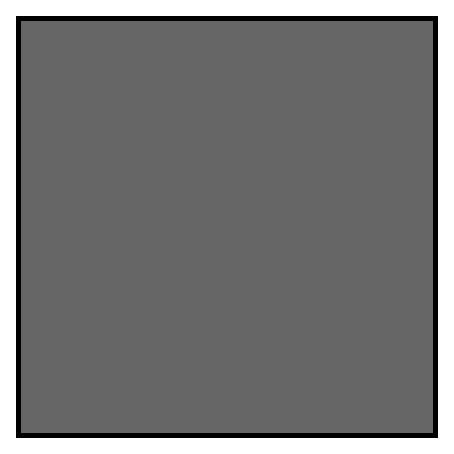
\includegraphics{example.eps}
%% figure caption is below the figure
%\caption{Please write your figure caption here}
%\label{fig:1}       % Give a unique label
%\end{figure}
%%
%% For two-column wide figures use
%\begin{figure*}
%% Use the relevant command to insert your figure file.
%% For example, with the graphicx package use
%  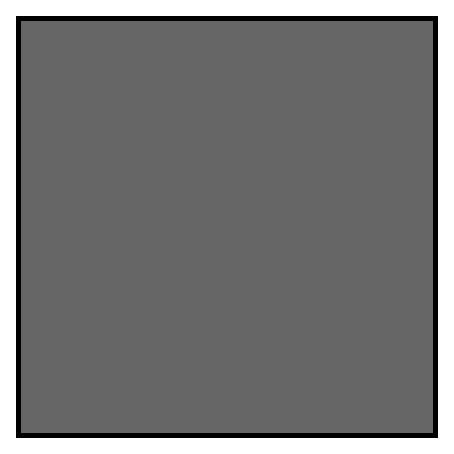
\includegraphics[width=0.75\textwidth]{example.eps}
%% figure caption is below the figure
%\caption{Please write your figure caption here}
%\label{fig:2}       % Give a unique label
%\end{figure*}
%%
%% For tables use
%\begin{table}
%% table caption is above the table
%\caption{Please write your table caption here}
%\label{tab:1}       % Give a unique label
%% For LaTeX tables use
%\begin{tabular}{lll}
%\hline\noalign{\smallskip}
%first & second & third  \\
%\noalign{\smallskip}\hline\noalign{\smallskip}
%number & number & number \\
%number & number & number \\
%\noalign{\smallskip}\hline
%\end{tabular}
%\end{table}

% -------------------- Acknowledgements ----------------------- %
%\begin{acknowledgements}
%If you'd like to thank anyone, place your comments here
%and remove the percent signs.
%\end{acknowledgements}



% -------------------- References ----------------------- %
% TODO: alle unten angegbenen Stile machen ganz komische Sachen
% Wer weiß, wie wir das fixen, bitte machen und oben \usepackage{natbib}
% und \bibliographystyle{plain} raus nehmen
% BibTeX users please use one of
%\bibliographystyle{spbasic}      % basic style, author-year citations
%\bibliographystyle{spmpsci}      % mathematics and physical sciences
%\bibliographystyle{spphys}       % APS-like style for physics
\bibliography{NAC-bibliography.bib}   % name your BibTeX data base

\end{document}

